\documentclass[9pt,a4paper]{extarticle}

% 引入中文支持及常用宏包
\usepackage[UTF8]{ctex}
\usepackage[left=1.2cm, right=1.2cm, top=0.8cm, bottom=1.0cm]{geometry}
\usepackage{enumitem}
\usepackage{titlesec}
\usepackage{hyperref}
\usepackage{xcolor}
\usepackage{graphicx}
\usepackage{tikz}

% ========== 紧凑行距：在保持 9pt 可读性的同时容纳五段科研经历 ==========
\linespread{1.18}

% 电子科技大学官方横向校标中的主蓝色
\definecolor{uestcblue}{HTML}{004098}

% 颜色与链接设置
\hypersetup{
    colorlinks=true,
    linkcolor=uestcblue,
    filecolor=uestcblue,
    urlcolor=uestcblue,
}

% ========== 投稿中徽章颜色 ==========
\definecolor{badgebg}{HTML}{FEF3C7}
\definecolor{badgeborder}{HTML}{F59E0B}
\definecolor{badgetext}{HTML}{92400E}

% 投稿中徽章命令
\newcommand{\submission}[1]{%
    \tikz[baseline=(text.base)]{%
        \node[
            fill=badgebg,
            draw=badgeborder,
            line width=0.4pt,
            rounded corners=2pt,
            inner xsep=4pt,
            inner ysep=1.2pt,
        ] (text) {\textbf{\color{badgetext}\small #1}};%
    }%
}

% ---------- 一级标题矢量图标（TikZ 路径，放大不失真） ----------
\newcommand{\educationicon}{%
    \tikz[baseline=-0.22em,x=1.08em,y=1.08em,line width=0.07em,line cap=round,line join=round]{%
        \draw[uestcblue] (0,0.18)--(0.50,0.40)--(1,0.18)--(0.50,-0.04)--cycle;
        \draw[uestcblue] (0.20,0.10)--(0.20,-0.10) .. controls (0.38,-0.27) and (0.62,-0.27) .. (0.80,-0.10)--(0.80,0.10);
        \draw[uestcblue] (1,0.18)--(1,-0.14);
        \fill[uestcblue] (1,-0.18) circle (0.055);
    }%
}
\newcommand{\researchicon}{%
    \tikz[baseline=-0.25em,x=0.94em,y=0.94em,line width=0.07em,line cap=round,line join=round]{%
        \draw[uestcblue] (0.34,0.42)--(0.34,0.10)--(0.12,-0.28) .. controls (0.04,-0.43) and (0.18,-0.48) .. (0.50,-0.48) .. controls (0.82,-0.48) and (0.96,-0.43) .. (0.88,-0.28)--(0.66,0.10)--(0.66,0.42);
        \draw[uestcblue] (0.27,0.42)--(0.73,0.42);
        \draw[uestcblue] (0.22,-0.18) .. controls (0.36,-0.10) and (0.64,-0.26) .. (0.78,-0.18);
    }%
}
\newcommand{\skillsicon}{%
    \tikz[baseline=-0.25em,x=0.94em,y=0.94em,line width=0.08em,line cap=round,line join=round]{%
        \draw[uestcblue] (0.31,0.34)--(0.04,0)--(0.31,-0.34);
        \draw[uestcblue] (0.69,0.34)--(0.96,0)--(0.69,-0.34);
        \draw[uestcblue] (0.59,0.42)--(0.41,-0.42);
    }%
}
\newcommand{\awardicon}{%
    \tikz[baseline=-0.25em,x=0.94em,y=0.94em,line width=0.07em,line cap=round,line join=round]{%
        \draw[uestcblue] (0.22,0.38)--(0.29,-0.01) .. controls (0.32,-0.18) and (0.42,-0.24) .. (0.50,-0.24) .. controls (0.58,-0.24) and (0.68,-0.18) .. (0.71,-0.01)--(0.78,0.38)--cycle;
        \draw[uestcblue] (0.23,0.28) .. controls (0.02,0.28) and (0.02,-0.03) .. (0.30,-0.06);
        \draw[uestcblue] (0.77,0.28) .. controls (0.98,0.28) and (0.98,-0.03) .. (0.70,-0.06);
        \draw[uestcblue] (0.50,-0.24)--(0.50,-0.42);
        \draw[uestcblue] (0.31,-0.42)--(0.69,-0.42);
    }%
}

% 自定义 section 样式：校标蓝标题与分隔线
\titleformat{\section}{\large\bfseries\raggedright\color{uestcblue}}{}{0em}{}[\color{uestcblue}\titlerule]
\titlespacing{\section}{0pt}{4pt}{3pt}

% 段落间距
\setlength{\parskip}{1pt}

% ---------- 科研项目方向行：右向矢量箭头、领域与时间 ----------
\newcommand{\projecticon}{%
    \tikz[baseline=-0.03em,x=0.90em,y=1.30em,line join=round]{%
        \fill[black!72] (0,0.42)--(0.65,0.21)--(0,0)--(0.15,0.21)--cycle;
    }%
}
\newcommand{\projectheading}[2]{%
    \noindent\projecticon\hspace{0.28em}\textbf{#1}\hfill\textbf{#2}\par\vspace{2pt}
}
\newcommand{\projectseparator}{%
    \par\vspace{3pt}%
    {\color{uestcblue!28}\hrule height 0.35pt}%
    \vspace{2pt}%
}

% ---------- 科研经历条目宏：方向与时间一行，论文标题独占一行 ----------
\newcommand{\researchentry}[3]{%
    \projectheading{#1}{#2}
    \noindent{\color{uestcblue}\textbf{#3}}\\[3pt]
}

% ---------- 同一科研经历下的多篇长标题论文：第二行右侧放状态与作者身份 ----------
\newcommand{\paperentry}[4]{%
    \noindent{\color{uestcblue}\textbf{#1}}\par
    \noindent{\color{uestcblue}\textbf{#2}}\hfill\mbox{#3\quad\textbf{#4}}\par\vspace{3pt}
}

\begin{document}
\pagestyle{empty}

% ==================== 头部联系方式 ====================
\noindent
\begin{minipage}[c][2.2cm][c]{0.295\textwidth}
    \raggedright
    
\includegraphics[width=5.0cm]{assets/uestc-horizontal-logo.png}
\end{minipage}%
\begin{minipage}[c][2.2cm][c]{0.515\textwidth}
    \centering
    \textbf{\huge 江浩} \\[4pt]
    \fontsize{10pt}{12pt}\selectfont
    \textbf{邮箱：}\href{mailto:Haolalala24@outlook.com}{Haolalala24@outlook.com}
    \quad | \quad
    \textbf{电话：}18728262751 \\[2pt]
    \textbf{GitHub：}\href{https://github.com/Haohaha-11}{Haohaha-11}
    \quad | \quad
    \textbf{个人主页：}\href{https://haohaha-11.github.io/}{haohaha-11.github.io}
\end{minipage}%
\begin{minipage}[c][2.2cm][c]{0.18\textwidth}
    \raggedleft
    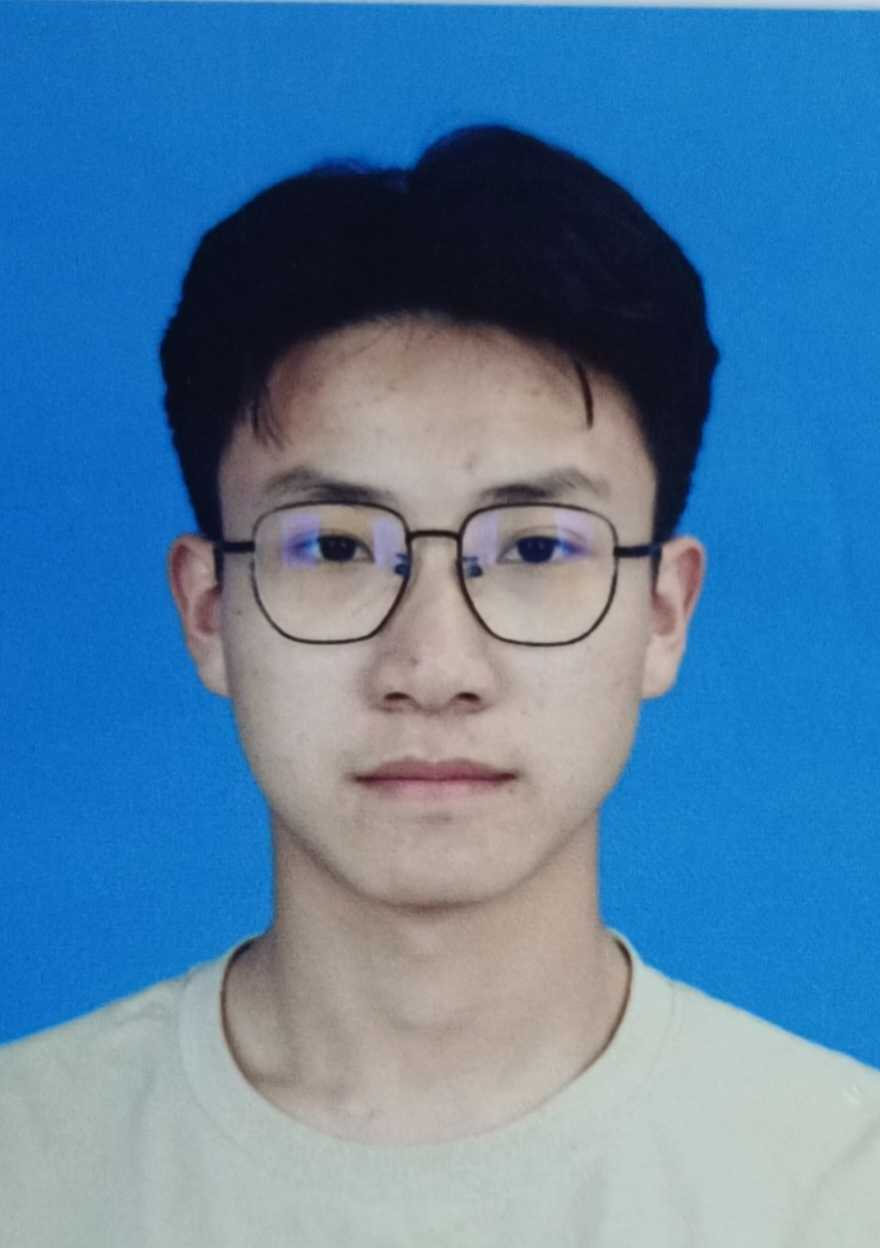
\includegraphics[height=2.2cm]{assets/portrait-user.jpg}
\end{minipage}
\vspace{2pt}

% ==================== 教育背景 ====================
\section*{\educationicon\hspace{0.38em}教育背景}
\noindent
\textbf{电子科技大学 \quad 英才实验学院（荣誉学院）} \hfill \textbf{2024.9 - 2028.6} \\
\textbf{专业：}数理基础科学（“成电英才计划”拔尖创新人才实验班）\quad \textbf{方向：}人工智能 \\ \quad \textbf{GPA: 3.96/4.0 \quad 加权均分：91.55 \quad 专业排名：2/24 \quad CET-4: 581 \quad CET-6: 561} \\
\textbf{核心课程：}高等微积分、高等代数与几何、大学物理、概率论与数理统计、机器学习等。

% ==================== 科研经历 ====================
\section*{\researchicon\hspace{0.38em}科研经历}

\researchentry{Computational Pathology \& Multiple Instance Learning\quad 计算病理与多示例学习}{2025.3 - 2025.8}{CKMIL: Cascaded Key-Instance Attention Multiple Instance Learning for Histopathology Whole Slide Image Analysis {\normalfont\href{https://haoceanlab.cn/pdfs/ckmil-aaai-26.pdf}{[pdf]}}{\normalfont\color{black}\hfill\mbox{Submitted to AAAI 2026\quad\textbf{第一作者}}}}
\textbf{指导教师：}电子科技大学 \quad 数学科学学院 \quad 邓良剑教授 \qquad 香港科技大学 \quad 陈浩助理教授
\begin{itemize}[leftmargin=*, nosep, itemsep=2pt]
    \item 针对病理全切片图像（WSI）关键诊断信号稀疏、全局交互易稀释关键信息的问题，提出级联关键实例注意力框架 CKMIL，以关键实例引导高效依赖建模；在 BRACS 与 TCGA 多队列癌症分型和生存预测任务上取得领先性能。
    \item 个人贡献：项目负责人，统筹研究进度，参与数据处理、方法构思、实验与论文撰写，主导项目全流程推进。
\end{itemize}
\projectseparator
\projectheading{LVLM Safety \& Jailbreak Attacks\quad 多模态大模型安全与越狱攻击}{2025.9 - 2025.12}
\paperentry{Persuasion in Scene: A Multi-Agent Typographic Jailbreak Crew against Large Vision-Language Models}{{\normalfont\href{https://haoceanlab.cn/pdfs/persuasion-in-scene-cvpr-2026.pdf}{[pdf]}}}{Submitted to CVPR 2026}{共同第一作者}
\paperentry{Models as Lego Builders: Assembling Malice from Benign Blocks via Semantic Blueprints}{{\normalfont\href{https://arxiv.org/pdf/2603.07590}{[pdf]}}}{Accepted by CVPR 2026}{第三作者}
\begin{itemize}[leftmargin=*, nosep, itemsep=2pt]
    \item 围绕 LVLM 黑盒越狱安全，提出多智能体跨模态协同框架 PIS 与基于语义槽填充漏洞的单次、免优化攻击框架 StructAttack；在主流开闭源 LVLM 上取得领先攻击成功率，揭示场景排印与结构化视觉提示的安全风险。
    \item \textbf{个人贡献：}作为 PIS 工作共同第一作者，核心参与研究构思、方法设计、实验推进与论文撰写；作为 StructAttack 工作第三作者，负责方法在 SafeBench 数据集上的适配与评测实验。
\end{itemize}
\projectseparator
\projectheading{Long-Context Test-Time Training\quad 长上下文测试时训练}{2026.1 - 2026.8}
\noindent{\color{uestcblue}\textbf{SPLIT: Write to Learn, Query to Retrieve in Long-Context Test-Time Training}}\hfill\mbox{Submitted to ICLR 2027\quad\textbf{第一作者}}\par\vspace{3pt}
\begin{itemize}[leftmargin=*, nosep, itemsep=2pt]
    \item 揭示长上下文测试时训练中内容归纳与稀疏检索的更新冲突，从 Where to Update 出发，提出双路径框架 SPLIT，以中层 MLP“写”路径学习可复用结构、深层 Query“读”路径增强长程检索；在 RULER、HELMET-ICL 与 LongBench 上取得显著提升。
    \item \textbf{个人贡献：}项目负责人，设计 Where、When、How to TTT 预实验并提出核心 Idea，推动方法从后训练方案向 Train-free 验证框架调整，负责全流程实验与论文撰写。
\end{itemize}
\projectseparator
\projectheading{Pathology Foundation Models \& Efficient WSI Analysis\quad 病理基础模型与高效全切片分析}{2025.12 - 至今}
\paperentry{From Full-Bag Diagnosis to Budgeted Patch Selection: Role-Decoupled Benchmarking and Adaptation of}{Pathology Foundation Models in Whole-Slide Imaging}{Expected Submission to IEEE TMI 2027}{第一作者}
\noindent\textbf{指导教师：}电子科技大学 \quad 数学科学学院 \quad 邓良剑教授 \qquad 香港科技大学 \quad 陈浩助理教授
\begin{itemize}[leftmargin=*, nosep, itemsep=2pt]
    \item 从病理图像压缩出发，发现部分形态学任务无需依赖图像重建，并将其归因于病理图像的高度冗余性与基础模型（FM）的鲁棒性；基于这两项性质，研究 Selector$\times$Consumer 场景下 FM 的能力解耦，并提出适配修复方案。
\end{itemize}
\projectseparator
\projectheading{Multimodal Post-Training \& Chain-of-Thought Reasoning\quad 多模态模型后训练与思维链推理}{2026.4 - 至今}
\paperentry{Seeing Again, Seeing Differently: ReMAP for Reasoning-Time Visual Memory Beyond One-Shot Encoding}{}{Submitted to ICLR 2027}{第一作者}
\begin{itemize}[leftmargin=*, nosep, itemsep=2pt]
    \item 通过预实验量化一次性视觉编码瓶颈：随长链推理推进，初始视觉证据的因果影响持续衰减；固定特征回放虽可恢复已保留信息，却无法补回首次编码遗漏的关键证据，形成 replay ceiling。受感知循环理论启发，提出 ReMAP 推理时自适应视觉工作空间，由当前推理状态在 Continue、Global Reorientation 与 Local Replay 间调节感知范围，以全局重定向缓解局部固着、恢复场景一致性，以局部回放返回原始像素并重编码细节证据，最终由模型按需 invoke 相应的 latent memory 支持后续推理。
\end{itemize}

% ==================== 专业技能 ====================
\section*{\skillsicon\hspace{0.38em}专业技能}
\begin{itemize}[leftmargin=*, nosep, itemsep=2pt]
    \item \textbf{编程与工具:} Python；熟练使用 PyTorch、Linux、Git、LaTeX、Codex、Claude Code；具备 Idea 验证、实验统筹与论文写作能力。
    \item \textbf{深度学习:} 熟悉 Transformer、Mamba 架构；具备多模态大模型测试时训练、后训练及系统评测经验；数理、学术英语基础扎实。
\end{itemize}

% ==================== 荣誉奖项 ====================
\section*{\awardicon\hspace{0.38em}荣誉奖项}
\begin{itemize}[leftmargin=*, nosep, itemsep=2pt]
    \item 电子科技大学优秀学生奖学金 \quad 一等 \hfill \textbf{2025年}
    \item 美国大学生数学建模竞赛（MCM/ICM） \quad Meritorious Winner（一等奖） \hfill \textbf{2026年}
\end{itemize}

\end{document}
